\chapter{Bubble dynamics}
\label{chap:bubble}
The dynamic behaviour of the bubble is modelled with a Rayleigh-Plesset-type (RP) model, assuming spherical symmetry. This requires to choose a suitable RP-type model (Section \ref{sec:rpmodels}) and define appropriate conditions for the gas  (Section \ref{sec:gas}), the liquid (Section \ref{sec:liquid}), the interface (Section \ref{sec:interface}), as well as at infinity (Section \ref{sec:infinity}). The results that APECSS can write out based on the RP model are explained in Section \ref{sec:bubble_results}.

APECSS solves all ordinary differential equations (ODEs) associated with the bubble dynamics using the embedded RK5(4) scheme of \citet{Dormand1980}, whereby a fifth-order Runge-Kutta scheme is used to solve the ODEs and the corresponding fourth-order Runge-Kutta scheme is used to estimate the solution error. Based on this solution error, the time-step $\Delta t$ used to advance the solution of the ODEs is adapted. If the solution error of a newly computed solution in a time-step does not satisfy the error tolerance, the solution is rewound and recomputed with a smaller $\Delta t$ (cf. sub-iteration), adapted based on the solution error of the previous attempt. 

\vspace{0.8em}

\noindent
\begin{tabular}{p{0.12\textwidth} p{0.32\textwidth} p{0.45\textwidth}}
    \textbf{Section} &\textbf{Command} & \textbf{Description} 
\vspace{1mm} \\ \hline
{\tt BUBBLE} & {\tt InitialRadius <float>} & The initial radius $R_0$ of the bubble.\\ 
 & {\tt PressureAmbient <float>} & The ambient pressure $p_0$.\\ 
 & {\tt InitialGasPressure <float>} & The initial gas pressure $p_{\mathrm{G},0}$, if different from $p_0$ or the corresponding Laplace pressure.\\ 
{\tt ODESOLVER} & {\tt RK 7M} & Minimum truncation (7M) coefficients of the RK5(4) scheme of \citet{Dormand1980}. This is the default.\\ 
& {\tt RK 7S} & Stability optimized (7S) coefficients of the RK5(4) scheme of \citet{Dormand1980}.\\ 
& {\tt Tolerance <float>} & The desired solution tolerance.\\ 
& {\tt MinTimeStep <float>} & Minimum time-step $\Delta t$.\\ 
& {\tt MaxTimeStep <float>} & Maximum time-step $\Delta t$.\\ 
& {\tt MaxSubIterations <float>} & Maximum number of sub-iterations in a given time-step.\\ 
 \hline
\end{tabular} \vspace{1em}

\section{Rayleigh-Plesset models}
\label{sec:rpmodels}

APECSS offers four RP-type models to simulate pressure-driven bubble dynamics: the standard Rayleigh-Plesset model without and with acoustic radiation damping, the Keller-Miksis model and the Gilmore model.

\vspace{0.8em}

\noindent
\begin{tabular}{p{0.12\textwidth} p{0.32\textwidth} p{0.45\textwidth}}
    \textbf{Section} &\textbf{Command} & \textbf{Description} 
\vspace{1mm} \\ \hline
{\tt BUBBLE} & {\tt RPModel RP} & Standard Rayleigh-Plesset model, Eq.~\eqref{eq:standardRP}. This is the default.\\ 
 & {\tt RPModel RPAR} & Rayleigh-Plesset model including acoustic radiation damping, Eq.~\eqref{eq:modRP}.\\ 
 & {\tt RPModel KM} & Keller-Miksis model, Eq.~\eqref{eq:keller}.\\ 
 & {\tt RPModel Gilmore} & Gilmore model, Eq.~\eqref{eq:gilmore}.\\ 
 \hline
\end{tabular} \vspace{1em}

\noindent The standard Rayleigh-Plesset (RP) model is given as \citep{Lauterborn2010}
\begin{equation}
R \ddot{R} + \frac{3}{2} \dot{R}^2 = \frac{p_\text{L} - p_\infty}{\rho_{\ell,\mathrm{ref}}},
\label{eq:standardRP}
\end{equation}
where $R$ is the bubble radius, $p_\text{L}$ is the pressure of the liquid at the bubble wall, $p_\infty$ is the pressure of the liquid in the far field, $p_\text{G}$ is the pressure of the gas inside the bubble and $\rho_{\ell,\mathrm{ref}}$ is the {\it constant} density of the liquid.

To incorporate acoustic radiation in the liquid and the associated damping, the modified Rayleigh-Plesset model is given as \citep{Brenner2002}
\begin{equation}
R \ddot{R} + \frac{3}{2} \dot{R}^2 = \frac{p_\text{L} - p_\infty}{\rho_{\ell,\mathrm{ref}}} + \frac{R \, \dot{p}_\text{G}}{\rho_{\ell,\mathrm{ref}} \, c_{\ell,\mathrm{ref}}} ,
\label{eq:modRP}
\end{equation}
where $c_{\ell,\mathrm{ref}}$ is the \textit{constant} reference speed of sound of the liquid. The last term on the right-hand side accounts for acoustic radiation in the liquid.
This modified RP model is frequently used to simulate medical ultrasound applications \citep{Versluis2020} as well as sonoluminescence \citep{Brenner2002}.
It follows directly from the Keller-Miksis model, Eq.~(\ref{eq:keller}), which incorporates the compressibility of the liquid, by assuming the Mach number of the bubble wall is vanishingly small, $M_\ell = \dot{R}/c_{\ell,\mathrm{ref}} \simeq 1$. Eq.~(\ref{eq:modRP}) is, consequently, only valid for small Mach numbers $M_\ell \ll 1$ \citep{Neppiras1980, Prosperetti1986}.

The Keller-Miksis model \citep{Keller1980, Prosperetti1986}, which incorporates the compressibility of the liquid to first order, is given as
\begin{equation}
\left(1 - \frac{\dot{R}}{c_{\ell,\mathrm{ref}}}\right) R \ddot{R} + \frac{3}{2} \left(1 - \frac{\dot{R}}{3\, c_{\ell,\mathrm{ref}}}\right) \dot{R}^2 =  \left(1 + \frac{\dot{R}}{c_{\ell,\mathrm{ref}}}\right) \frac{p_\text{L} - p_\infty}{\rho_{\ell,\mathrm{ref}}} + R \, \frac{\dot{p}_\text{L} - \dot{p}_\infty}{\rho_{\ell,\mathrm{ref}} \, c_{\ell,\mathrm{ref}}} ,
\label{eq:keller}
\end{equation}
where $c_{\ell,\mathrm{ref}}$ is the speed of sound of the liquid. Both $\rho_{\ell,\mathrm{ref}}$ and $c_{\ell,\mathrm{ref}}$ are assumed to be constant, limiting the Keller-Miksis model to moderate liquid pressures ($p_\mathrm{L} \lesssim 10^8 \, \mathrm{Pa}$).

Based on the Kirkwood-Bethe hypothesis \citep{Kirkwood1942,Cole1948}, \citet{Gilmore1952} derived a second-order ordinary differential equation describing the radial dynamics of a bubble in a compressible liquid, %given as
\begin{equation}
  \left( 1 - \frac{\dot{R}}{c_\text{L}} \right) R \ddot{R} + \frac{3}{2} \left( 1 - \frac{\dot{R}}{3 c_\text{L}} \right) \dot{R}^2  = \left( 1 + \frac{\dot{R}}{c_\text{L}} \right) H + \left( 1- \frac{\dot{R}}{c_\text{L}} \right) \frac{R \dot{H}}{c_\text{L}}, \label{eq:gilmore}
\end{equation} 
where $c_\mathrm{L}$ is the speed of sound of the liquid at the bubble wall, $H = h_\text{L} - h_\infty$ is the enthalpy difference between the bubble wall and infinity, and $\dot{H} = \dot{h}_\text{L} - \dot{h}_\infty$ is the derivative of $H$. The enthalpy $h$ and the speed of sound $c$ are defined by an appropriate equation of state as a function of pressure, with $h_\text{L} = h(p_\text{L})$, $h_\infty = h(p_\infty)$ and $c_\text{L} = c(p_\text{L})$, as detailed in \ref{sec:liquid}.

\section{The gas}
\label{sec:gas}

In APECSS, every bubble contains a gas, which requires to select an appropriate equation of state and define meaningful properties.

\vspace{0.8em}

\noindent
\begin{tabular}{p{0.1\textwidth} p{0.36\textwidth} p{0.49\textwidth}}
    \textbf{Section} &\textbf{Command} & \textbf{Description} 
\vspace{1mm} \\ \hline
{\tt GAS} & {\tt EoS IG} & Ideal gas equation of state. This is the default.\\ 
& {\tt EoS HC} & Ideal gas equation of state with van-der-Waals hardcore.\\ 
& {\tt EoS NASG} & Noble-Abel-stiffened-gas equation of state.\\
& {\tt PolytropicExponent <float>} & Polytropic exponent $\Gamma_\text{g}$.\\
& {\tt ReferencePressure <float>} & Reference pressure $p_\text{g,ref}$.\\
& {\tt ReferenceDensity <float>} & Reference density $\rho_\text{g,ref}$.\\
& {\tt CoVolume <float>} & Co-volume $b_\text{g}$.\\
& {\tt TaitPressureConst <float>} & Pressure constant $B_\text{g}$.\\
& {\tt MolecularWeight <float>} & Molecular weight $\mathcal{M}_{\text{g}}$ of the gas.\\
& {\tt MolecularDiameter <float>} & Molecular kinematic diameter $\mathcal{D}_{\text{g}}$ of the gas.\\
{\tt BUBBLE} & {\tt HardcoreRadius <float>} & Hardcore radius $r_\text{hc}$.\\
 \hline
\end{tabular} \vspace{1em}


Using the ideal gas EoS, the pressure and its derivative are given as
\begin{align}
  p_\text{G} &= p_\text{G,ref} \left(\frac{R_0}{R}\right)^{3 \Gamma_\text{g}}\\
  \dot{p}_\text{G} &= -3 \, \frac{p_\text{G} \, \Gamma_\text{g} \, \dot{R}}{R},\\
\end{align}
including a van-der-Waals hardcore (HC) in the ideal gas model, the pressure and its derivative follow as
\begin{align}
  p_\text{G} &= p_\text{G,ref} \left(\frac{R_0^3-r_\text{hc}^3}{R^3-r_\text{hc}^3}\right)^{\Gamma_\text{g}}\\
  \dot{p}_\text{G} &= -3 \, \frac{p_\text{G} \, \Gamma_\text{g} \, R^2 \, \dot{R}}{R^3-r_\text{hc}^3},
\end{align}
and using the Noble-Abel-stiffened-gas (NASG) EoS, the pressure and its derivative are \citep{Denner2021}
\begin{align}
  p_\text{G} &= (p_\text{G,ref} + B_\text{g}) \left[\frac{\rho_\text{g} \, (1-b_\text{g} \, \rho_\text{g,ref})}{\rho_\text{g,ref} \, (1- b_\text{g} \, \rho_\text{G})} \right]^{\Gamma_\text{g}} - B_\text{g}\\
  \dot{p}_\text{G} &= \frac{\dot{\rho}_\text{G} \, \Gamma_\text{g} \left(p_\text{G} + B_\text{g} \right)}{\rho_\text{G} \left(1- b_\text{g} \, \rho_\text{G} \right)},
\end{align}
where $\Gamma_\mathrm{g}$ is the polytropic exponent, $r_\mathrm{hc}$ is the hardcore radius, $b_\mathrm{g}$ is the co-volume and $B_\mathrm{g}$ is a pressure constant.

Assuming mass conservation, the gas density and its derivative are given by 
\begin{align}
  \rho_\text{G} &= \rho_\text{g,ref} \left(\frac{R_0}{R}\right)^3 \label{eq:rhoG}\\
  \dot{\rho}_\text{G} &= -3 \, \rho_\text{G}\, \frac{\dot{R}}{R}. \label{eq:dot_rhoG}
\end{align}

The hardcore radius $r_\mathrm{hc}$ and the co-volume $b_\mathrm{g}$ are set by default to $-1$. If the {\tt HC} or {\tt NASG} model is chosen, the user has to pass values for the hardcore radius $r_\mathrm{hc}$ or the co-volume $b_\mathrm{g}$, respectively. Alternatively, the molecular weight $\mathcal{M}_{\text{g}}$ and the molecular kinematic diameter $\mathcal{D}_{\text{g}}$ of the gas may be defined instead of $r_\mathrm{hc}$ or $b_\mathrm{g}$; APECSS then computes the correct co-volume $b_\mathrm{g}$ or, based on the bubble size, hardcore radius $r_\mathrm{hc}$. Assuming the molecular weight $\mathcal{M}_{\text{g}}$, the bubble contains 
\begin{equation}
    N_\mathrm{G} = N_\mathrm{A} \, \frac{\rho_{\mathrm{G},0} V_0}{\mathcal{M}_{\text{g}}} 
\end{equation}
molecules, where $N_\mathrm{A}$ is the Avogadro constant (see macro {\tt APECSS\_AVOGADRO}), $\rho_{\mathrm{G},0}$ is the initial gas density and $V_0$ is the initial bubble volume. As per the molecular kinetic diameter $\mathcal{D}_{\text{g}}$ of the gas molecules, the volume of each molecule is
\begin{equation}
    V_\mathrm{mol} = \frac{\pi}{6} \, \mathcal{D}_{\text{g}}^3.
\end{equation}
The van-der-Waals hardcore radius is then readily defined as
\begin{equation}
    r_\mathrm{hc} = \sqrt[3]{\frac{3}{4 \pi} f_\mathrm{mol} \, V_\mathrm{mol} \, N_\mathrm{G}}
\end{equation}
and the co-volume of the gas is given as
\begin{equation}
    b_\mathrm{g} = f_\mathrm{mol} \, N_\mathrm{A} \, \frac{V_\mathrm{mol}}{\mathcal{M}_{\text{g}}}.
\end{equation}
The semi-empirical constant $f_\mathrm{mol}$ is based on the repulsive forces acting between the molecules \citep{Kontogeorgis2019}, and is typically taken to be $f_\mathrm{mol}=4$.


\section{The liquid}
\label{sec:liquid}

In the same way that every bubble contains a gas, in APECSS every bubble is surrounded by a liquid, which requires to select an appropriate equation of state and fluid type, as well as define meaningful properties.

\vspace{0.8em}

\noindent
\begin{tabular}{p{0.1\textwidth} p{0.35\textwidth} p{0.5\textwidth}}
    \textbf{Section} &\textbf{Command} & \textbf{Description} 
\vspace{1mm} \\ \hline
{\tt LIQUID} & {\tt EoS Tait} & The Tait EoS is applied to the liquid. Only relevant for the Gilmore model and acoustic emissions based on the Kirkwood-Bethe hypothesis.\\ 
& {\tt EoS NASG} & The Noble-Abel-stiffened-gas EoS is applied to the liquid. Only relevant for the Gilmore model and acoustic emissions based on the Kirkwood-Bethe hypothesis.\\ 
& {\tt LiquidType Newtonian} & Newtonian fluid. This is the default.\\ 
& {\tt LiquidType KelvinVoigt} & Kelvin-Voigt solid.\\ 
& {\tt LiquidType Zener} & Zener solid.\\ 
& {\tt LiquidType OldroydB} & Oldroyd-B (or upper-convected Maxwell) fluid.\\ 
& {\tt PolytropicExponent <float>} & Polytropic exponent $\Gamma_{\ell}$.\\
& {\tt ReferencePressure <float>} & Reference pressure $p_{\ell,\text{ref}}$.\\
& {\tt ReferenceDensity <float>} & Reference density $\rho_{\ell,\text{ref}}$.\\
& {\tt ReferenceSpeedofSound <float>} & Reference speed of sound $\rho_{\ell,\text{ref}}$.\\
& {\tt CoVolume <float>} & Co-volume $b_\ell$.\\
& {\tt TaitPressureConst <float>} & Pressure constant $B_\ell$.\\
& {\tt Viscosity <float>} & Newtonian viscosity $\mu_\ell$.\\
& {\tt PolymerViscosity <float>} & Polymer viscosity $\eta_\ell$ associated with viscoelasticity.\\
& {\tt ShearModulus <float>} & Shear modulus $G_\ell$ associated with viscoelasticity.\\
& {\tt RelaxationTime <float>} & Relaxation time $\lambda_\ell$ associated with viscoelasticity.\\
 \hline
\end{tabular} \vspace{1em}

The pressure at the bubble wall of a Newtonian liquid is given as
\begin{equation}
  p_\text{L} = p_\text{G} - \frac{2 \sigma}{R} - 4 \, \mu_\ell \frac{\dot{R}}{R}, \label{eq:pL}
\end{equation}
where $p_\text{G}$ is the gas pressure, see Section \ref{sec:gas}, $\sigma$ is the surface tension coefficient of the interface, see Section \ref{sec:interface}, and $\mu_\ell$ is the liquid (Newtonian) viscosity. The derivative of Eq.~\eqref{eq:pL} follows as
\begin{equation}
  \dot{p}_\mathrm{L} = \dot{p}_\mathrm{G} + \frac{2 \, \sigma \, \dot{R}}{R^2} + 4 \, \mu_\ell \left(\frac{\dot{R}^2}{R^2} - \frac{\ddot{R}}{R}\right).
  \label{eq:dotpL}
\end{equation}

\subsection{Equation of state}

For the Gilmore model \eqref{eq:gilmore} and the acoustic emissions based on the Kirkwood-Bethe hypothesis (see Section \ref{sec:emissionskb}), an equation of state (EoS) for the liquid has to be defined. Two EoS are currently available in APECSS: the Tait EoS and the NASG EoS. 

Since the seminal work of \citet{Gilmore1952}, the Tait EoS is traditionally used to describe the properties of the liquid in Eq.~\eqref{eq:gilmore}. The Tait EoS defines the density $\rho$, enthalpy $h$ and speed of sound $c$ as
\begin{align}
    \rho &= \rho_{\ell,\text{ref}} \left( \frac{p+B_\ell}{p_{\ell,\text{ref}}+B_\ell}\right)^{\frac{1}{\Gamma_\ell}} \label{eq:rho_Tait} \\
    h &= \frac{\Gamma_\ell}{\Gamma_\ell-1} \frac{p+B_\ell}{\rho} \label{eq:h_Tait} \\
    c &= \sqrt{(\Gamma_\ell -1) \, h}, \label{eq:c_Tait}
\end{align}
respectively, where $B_\ell$ is a pressure constant, $\Gamma_\ell$ is the polytropic exponent, $p_{\ell,\text{ref}}$ is the reference pressure and $\rho_{\ell,\text{ref}}$ is the reference density. For water, typical values are $\Gamma_\ell=7.15$, $B_\ell=3.046 \times 10^8 \, \text{Pa}$, $\rho_{\ell,\text{ref}} = 997 \, \mathrm{kg/m}^3$ and $p_{\ell,\text{ref}} = 10^5 \, \mathrm{Pa}$. 

Using the Noble-Abel stiffened-gas (NASG) EoS \citep{LeMetayer2016} instead of the Tait EoS, the fluid properties are defined as \citep{Denner2021}
 \begin{eqnarray}
    \rho &=& \frac{K_\ell \, (p+B_\ell)^{\frac{1}{\Gamma_\ell}}}{1+b_\ell \, K_\ell \,  (p+B_\ell)^{\frac{1}{\Gamma_\ell}}} \label{eq:rho_NASG}\\
      h &=& \frac{\Gamma_\ell}{\Gamma_\ell-1} \frac{p+B_\ell}{\rho} - \frac{\Gamma_\ell \, b_\ell}{\Gamma_\ell-1} \, (p+B_\ell) + b_\ell \, p \label{eq:h_NASG} \\
      c &=&\sqrt{\Gamma_\ell \, \frac{(p+B_\ell)}{\rho-b_\ell  \rho^2}},\label{eq:c_NASG}
    \end{eqnarray}
with $K_\ell = \rho_{\ell,\text{ref}}/[(p_{\ell,\text{ref}}+B_\ell)^{{1/\Gamma_\ell}} \ (1-b_\ell \rho_{\ell,\text{ref}})]$ describing a constant reference state, and where $b_\ell$ is the co-volume of the liquid molecules. The NASG EoS reduces to the Tait EoS for $b_\ell=0$. Appropriate properties for water have, for instance, been proposed by \citet{Chandran2019} as $\Gamma_\ell = 1.19$, $B_\ell = 6.2178 \times 10^{8} \, \mathrm{Pa}$, $b_\ell = 6.7212 \times 10^{-4} \, \mathrm{m}^3/\mathrm{kg}$, $\rho_{\ell,\text{ref}} = 997 \, \mathrm{kg/m}^3$ and $p_{\ell,\text{ref}} = 10^5 \, \mathrm{Pa}$.

\subsection{Viscoelasticity}

Currently, APECSS supports three widely-used models for viscoelastic media: the Kelvin-Voigt model, the Zener model and the Oldroyd-B model. While the Kelvin-Voigt model merely yields an additional term in the expression for the liquid pressure at the bubble wall, the Zener and Oldroyd-B models each require to solve two additional ODEs.

\subsubsection{Kelvin-Voigt model}

To model a Kelvin-Voigt medium, the elasticity of the medium is described by the additional term 
\begin{equation}
    \frac{4}{3} \, G_\ell \, \frac{R^3-R_0^3}{R^3}, \label{eq:KVterm}
\end{equation}
which contributes to Eq.~\eqref{eq:pL} to obtain
\begin{equation}
    p_\text{L} = p_\text{G} - \frac{2 \sigma}{R} - 4 \, \mu_\ell \frac{\dot{R}}{R} - \frac{4}{3} \, G_\ell \, \frac{R^3-R_0^3}{R^3}, \label{eq:pL_KV}
\end{equation}
where $G_\ell$ is the elastic shear modulus.
% The derivative of Eq.~\eqref{eq:KVterm} is given as
% \begin{equation}
%     \frac{\text{d}}{\text{d}t} \left(\frac{4}{3} \, G_\ell \, \frac{R^3-R_0^3}{R^3} \right) =  4 \, G_\ell \, \frac{R_0^3 \dot{R}}{R^4}.  \label{eq:dotKVterm}
% \end{equation}
The derivative of the liquid pressure at the bubble wall is then given as
\begin{equation}
    \dot{p}_\mathrm{L} = \dot{p}_\mathrm{G} + \frac{2 \, \sigma \, \dot{R}}{R^2} + 4 \, \mu_\ell \left(\frac{\dot{R}^2}{R^2} - \frac{\ddot{R}}{R}\right) - 4 \, G_\ell \, \frac{R_0^3 \dot{R}}{R^4}.
    \label{eq:dotpL_KV}
\end{equation}

\subsubsection{Zener model}

A more sophisticated viscoelastic model than the Kelvin-Voigt model is the Zener model, also known as standard linear solid model. With the Zener model, the stresses in the medium surrounding the bubble are incorporated in the liquid pressure at the bubble wall as \citep{Hua2013}
\begin{equation}
     p_\text{L} = p_\text{G} - \frac{2 \sigma}{R} + 3 \varsigma \label{eq:pL_Zener}
\end{equation}
where
\begin{equation}
    \varsigma= \int_R^\infty \frac{\tau_{rr}(r,t)}{r} \, \mathrm{d}r
\end{equation}
is an auxiliary variable associated with the $rr$-component of the viscous stress tensor $\boldsymbol{\tau}(r,t)$. The auxiliary stress variable is governed by
\begin{align}
    \lambda_\ell \dot{\varsigma} + \varsigma +\lambda_\ell \frac{\dot{R}}{R} {\tau}_{rr|R} &= - \frac{S}{3},  \label{eq:ode_varsigma}
\end{align}
with
\begin{equation}
    S = \frac{4}{3} G_\ell \left( 1- \frac{R_0^3}{R^3} \right) + 4 \mu_\ell \frac{\dot{R}}{R}
\end{equation}
the combined viscous and elastic contributions, where $\lambda_\ell$ is the relaxation time, $G_\ell$ is the shear modulus and $\mu_\ell$ the viscosity. The stress at the bubble wall, ${\tau}_{rr|R}$, evolves as
\begin{align}
    \lambda_\ell \dot{\tau}_{rr|R} + {\tau}_{rr|R} &= -S. \label{eq:ode_tau}
\end{align}

The question is now how to solve the ODEs for $\varsigma$ and $\tau_{rr}$ in such a way that we always obtain a meaningful result, even if $\lambda_\ell=0$. In order for a customary ODE solver to handle this correctly, we rearrange Eqs.~\eqref{eq:ode_varsigma} and \eqref{eq:ode_tau}. Under the discrete assumption
\begin{equation}
    \dot{\varsigma}  = \frac{\varsigma_{n+1}-\varsigma_n}{\Delta t},
\end{equation}
Eq.~\eqref{eq:ode_varsigma} becomes
\begin{equation}
    \lambda_\ell \frac{\varsigma_{n+1}-\varsigma_n}{\Delta t} + \varsigma_{n+1} +\lambda_\ell \frac{\dot{R}}{R} {\tau}_{rr|R} = - \frac{S}{3}
  \end{equation}
so that, after some further manipulation,
\begin{equation}
    \varsigma_{n+1} =  \varsigma_n + \Delta t \frac{- \dfrac{S}{3} - \lambda_\ell  \dfrac{\dot{R}}{R} {\tau}_{rr|R,n} - \varsigma_n}{\lambda_\ell + \Delta t}. \label{eq:varsigma_reformulated}
  \end{equation}
Similarly, Eq.~\eqref{eq:ode_tau} follows as
\begin{equation}
   {\tau}_{rr|R,n+1} = {\tau}_{rr|R,n} + \Delta t \frac{-S-{\tau}_{rr|R,n}}{\lambda_\ell + \Delta t}.
   \label{eq:tau_reformulated}
\end{equation}
Even in the limit $\lambda_\ell = 0$, we can now obtain a meaningful answer, that is Eq.~\eqref{eq:varsigma_reformulated} reduces to
\begin{equation}
    \varsigma = -\frac{S}{3}. \label{eq:varsigma_lambdaNull}
\end{equation}
After inserting Eq.~\eqref{eq:varsigma_lambdaNull} into Eq.~\eqref{eq:pL_Zener} we recover the Kelvin-Voigt model. For $\lambda_\ell = 0$, Eq.~\eqref{eq:tau_reformulated} becomes redundant.

\subsubsection{Oldroyd-B model}

The Oldroyd-B model is a widely used constitutive model for viscoelastic fluids. 
Following the work of \citet{Jimenez-Fernandez2005}, the liquid pressure at the bubble wall including the Oldroyd-B model is given as
\begin{equation}
     p_\text{L} = p_\text{G} - \frac{2 \sigma}{R} - 4 \mu_\ell \frac{\dot{R}}{R} + \mathcal{S} \label{eq:pL_OldroydB}.
\end{equation}
The polymer stress $\mathcal{S} = \mathcal{S}_1 + \mathcal{S}_2$ is split into two constitutive ODEs,
\begin{align}
    \lambda_\ell \dot{\mathcal{S}}_1 + \mathcal{S}_1 + 4 \lambda_\ell \frac{\dot{R}}{R} \mathcal{S}_1 &= - 2 \eta_\ell \frac{\dot{R}}{R}\\  
    \lambda_\ell \dot{\mathcal{S}}_2 + \mathcal{S}_2 +  \lambda_\ell \frac{\dot{R}}{R} \mathcal{S}_2 &= - 2 \eta_\ell \frac{\dot{R}}{R}
\end{align}
where $\eta_\ell$ is the polymer viscosity.
These ODEs are reformulated in a similar manner as for the Zener model shown above, to yield
\begin{align}
    \mathcal{S}_{1,n+1} &= \mathcal{S}_{1,n} + \Delta t \frac{-\left(4 \lambda_\ell \dfrac{\dot{R}}{R}+1\right) \mathcal{S}_{1,n}- 2 \eta_\ell \dfrac{\dot{R}}{R}}{\lambda_\ell+\Delta t} \label{eq:ode_oldroydB1disc} \\
    \mathcal{S}_{2,n+1} &= \mathcal{S}_{2,n} + \Delta t \frac{-\left(\lambda_\ell \dfrac{\dot{R}}{R}+1\right) \mathcal{S}_{2,n}- 2 \eta_\ell \dfrac{\dot{R}}{R}}{\lambda_\ell+\Delta t}.\label{eq:ode_oldroydB2disc}
\end{align}
For $\lambda_\ell = 0$ Eqs.~\eqref{eq:ode_oldroydB1disc} and \eqref{eq:ode_oldroydB2disc} still give a meaningful result and reduce to a Newtonian fluid with $\mathcal{S} = - 4 \eta_\ell \dot{R}/R$.

\section{The interface}
\label{sec:interface}

APECSS readily supports the gas-liquid interface, also often referred to as the \textit{bubble wall},  to be either clean, for which only the surface tension coefficient has to be defined, or coated with a lipid monolayer.

\vspace{0.8em}

\noindent
\begin{tabular}{p{0.11\textwidth} p{0.44\textwidth} p{0.40\textwidth}}
    \textbf{Section} &\textbf{Command} & \textbf{Description} 
\vspace{1mm} \\ \hline
{\tt INTERFACE} & {\tt SurfaceTensionCoeff <float> } & Surface tension coefficient $\sigma_\mathrm{c}$ of the clean interface.\\ 
& {\tt LipidCoatingModel None} & No lipid coating model is applied. This is the default.\\ 
& {\tt LipidCoatingModel Marmottant} & The lipid coating model of \citet{Marmottant2005} is applied.\\ 
& {\tt LipidCoatingModel Gompertz-Marmottant} & The continuous variant of the lipid coating model of Marmottant proposed by \citet{Guemmer2021} is applied.\\
& {\tt SigmaInit <float>} & Initial surface tension coefficient $\sigma_0$ of the lipid coating model at $R_0$.\\ 
& {\tt Elasticity <float>} & Elasticity $\chi$ of the lipid coating model.\\ 
& {\tt DilatationalViscosity <float>} & Dilatational viscosity $\kappa_\mathrm{s}$ of the lipid coating model.\\ 
 \hline
\end{tabular} \vspace{1em}

The influence of surface tension, the rheology of the lipid-monolayer coating and the viscous dissipation in the liquid is accounted for through the definition of the liquid pressure at the bubble wall, given as \citep{Marmottant2005}
\begin{equation}
p_\text{L} = p_\text{G} - \frac{2 \sigma}{R} - 4 \, \mu_\ell \frac{\dot{R}}{R} - 4 \, \kappa_\text{s} \frac{\dot{R}}{R^2} ,
\end{equation}
where $\sigma$ is the surface tension coefficient, $\mu_\ell$ is the dynamic viscosity of the liquid and $\kappa_\text{s}$ is the surface dilatational viscosity of the lipid monolayer.

A clean gas-liquid interface has a surface tension coefficient of $\sigma = \sigma_\text{c}$ and a surface dilatational viscosity of $\kappa_\text{s} = 0$. 

Using the model of \citet{Marmottant2005} to describe a lipid monolayer coating of the interface, the surface tension is defined as
\begin{equation}
\sigma =
\begin{cases}
0 & \text{for} \ R \leq R_\text{buck} \\
\chi \left(\dfrac{R^2}{R_\text{buck}^2} - 1 \right) & \text{for} \ R_\text{buck} < R < R_\text{rupt} \\
\sigma_\text{c} & \text{for} \ R \geq R_\text{rupt}
\end{cases} \label{eq:sigma_marmottant}
\end{equation}
where $\chi$ is the surface elasticity of the lipid monolayer, the buckling radius is \citep{Overvelde2010}
\begin{equation}
R_\text{buck} = \frac{R_0}{\sqrt{1 + \sigma_0/\chi}}, 
\label{eq:Rbuck}
\end{equation}
where $\sigma_0$ is the surface tension coefficient of the lipid-coated bubble at $R=R_0$, and the rupture radius is
\begin{equation}
R_\text{rupt} = R_\text{buck} \, \sqrt{1+\frac{\sigma_\text{c}}{\chi}}.
\label{eq:Rrupt}
\end{equation} 

The radius-dependent surface tension coefficient of the Marmottant model \citep{Marmottant2005}, defined in Eq.~(\ref{eq:sigma_marmottant}), contains two discontinuities at $R=R_\text{buck}$ and $R=R_\text{rupt}$. These discontinuities render the Marmottant model sensitive to the applied time-step when numerically solving the primary ordinary differential equation \citep{Versluis2020}. A continuously differentiable form of the Marmottant model a Gompertz function of the form $f(x) = a \, \text{e}^{-b \, \text{e}^{-c x}}$, a special case of the generalized logistics function, was proposed by \citet{Guemmer2021}. Using this Marmottant-Gompertz model, the surface tension coefficient is defined as
\begin{equation}
\sigma = \sigma_\text{c} \, \text{e}^{-b \, \text{e}^{c (1-R/R_\text{buck})}}, \label{eq:sigma_gompertz}
\end{equation}
with
\begin{equation}
    b = - \frac{\ln (\sigma_0/\sigma_\text{c})}{\text{e}^{c(1-R_0/R_\text{buck})}}
\end{equation}
and
\begin{equation}
    c = \frac{2  \chi  \text{e}}{\sigma_\text{c}} \, \sqrt{1+\frac{\sigma_\text{c}}{2 \chi}}.
\end{equation}
The buckling radius $R_\text{buck}$ is given by Eq.~(\ref{eq:Rbuck}). 
The derivative of the surface tension coefficient follows as
\begin{equation}
\dot{\sigma} = \sigma \, b \, c \, \text{e}^{c (1-R/R_\text{buck})} \, \frac{\dot{R}}{R}.
\end{equation}

The Marmottant-Gompertz model reproduces the main features of the original Marmottant model \citep{Guemmer2021}, but with a smooth transition between the surface tension regimes, using the same set of input parameters ($\sigma_0$, $\sigma_\text{c}$, $\chi$) as the original Marmottant model.

\section{Infinity}
\label{sec:infinity}

The pressure at infinity, $p_\infty$, is used to apply a driving pressure difference for the bubble dynamics. Presently, APECSS readily supports a constant ambient pressure $p_\infty = p_0$, which may also be replaced by a pressure defined on-the-fly (e.g.~provided by a fluid dynamics solver running concurrently with APECSS), or a sinusoidal excitation. 

A sinusoidal excitation is defined as $p_\infty = p_0 - \Delta p_\mathrm{a} \, \sin(2 \pi f_\mathrm{a} t)$, where $f_\mathrm{a}$ and $\Delta p_\mathrm{a}$ are the frequency and pressure amplitude of the excitation. In order to use the sinusoidal excitation, the user has to allocate the pointer {\tt *Excitation}, in the structure {\tt APECSS\_Bubble} structure, with {\tt struct APECSS\_Excitation} and define the desired values for  $f_\mathrm{a}$ and $\Delta p_\mathrm{a}$. The example found in the folder {\tt example/ultrasound/} provides a template of how to do this.

\section{Results}
\label{sec:bubble_results}

The results of the bubble dynamics can be written to disk, if so desired by the user. Note that APECSS does \uline{not} write any results to disk unless it is specifically asked to do so.

\vspace{0.8em}

\noindent
\begin{tabular}{p{0.11\textwidth} p{0.28\textwidth} p{0.56\textwidth}}
    \textbf{Section} &\textbf{Command} & \textbf{Description} 
\vspace{1mm} \\ \hline
{\tt RESULTS} & {\tt Bubble} & Results of the bubble dynamics are written to file.\\ 
& {\tt OutputFreqRP <int>} & Results of the bubble dynamics are stored every so many time steps (default: 1).\\ 
& {\tt OutputPath <string>} & Path to the folder where all the results should be written in to (default: {\tt ./}).\\
& {\tt OutputDigits <int>} & Results are written out with as many digits (default: 6).\\
 \hline
\end{tabular} \vspace{1em}

For the bubble dynamics, the following quantities as a function of time are written into a text file, named by the employed RP model and (if applicable) the excitation parameters used:\vspace{-1em}
\begin{itemize}[noitemsep]
  \item Time-step number.
  \item Time, $t$.
  \item Time-step, $\Delta t$.
  \item Bubble radius, $R$.
  \item Velocity of the bubble wall, $\dot{R}$.
  \item Pressure of the gas, $p_\mathrm{G}$.
  \item Pressure of the liquid at the bubble wall, $p_\mathrm{L}$.
  \item Pressure of the liquid in the far field, $p_\infty$.
  \item Speed of sound of the liquid at the bubble wall, $c_\mathrm{L}$, if the Gilmore model is applied.
  \item The result of any additional user-defined ODE solved, if applicable.
\end{itemize}

The first line of the results file(s) lists the variables that were written out and their order. For instance, Figure \ref{fig:bubble_results} shows the output of the ``simple'' ultrasound-driven lipid-coated microbubble examples ({\tt \$APECSS\_DIR/examples/ultrasound/lipidcoated\_simple.apecss}).

\begin{figure}
    \centering
    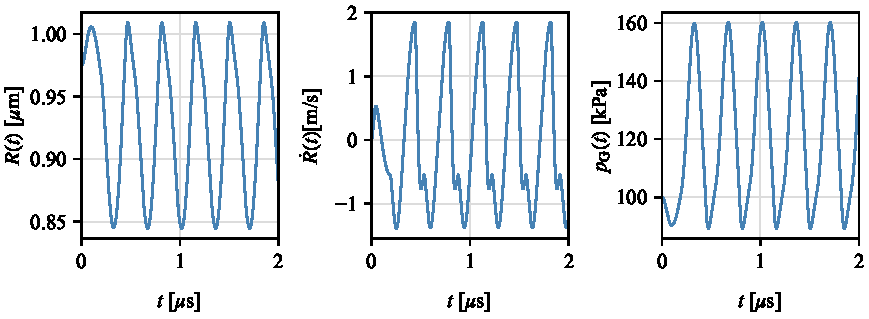
\includegraphics[width=\linewidth]{./figures/ultrasound_lipidcoated_simple.pdf}
    \caption{Temporal evolution of the radius $R(t)$, bubble wall velocity $\dot{R}(t)$ and gas pressure $p_\mathrm{G}(t)$ of a lipid-coated microbubble with initial radius $R_0 = 0.975 \, \upmu \mathrm{m}$, driven by ultrasound with a frequency of $2.9 \, \mathrm{MHz}$ and a pressure amplitude of $130 \, \mathrm{kPa}$, as previously considered by \citet{Marmottant2005}. This example can be found in {\tt \$APECSS\_DIR/examples/ultrasound}, called {\tt lipidcoated\_simple}.}
    \label{fig:bubble_results}
\end{figure}